\documentclass{beamer}

% Make each \item a separate slide
% \beamerdefaultoverlayspecification{<+->}

\usetheme{metropolis}           % Use metropolis theme

\usepackage{graphicx}
\usepackage{animate}
\usepackage{hyperref}

% Make LaTeX math render using normal fonts
\usefonttheme{professionalfonts} % required for mathspec
\usepackage{mathspec}
\setsansfont[BoldFont={Fira Sans},
Numbers={OldStyle}]{Fira Sans Light}
\setmathsfont(Digits)[Numbers={Lining, Proportional}]{Fira
Sans Light}

\title{WaveNet: A Generative Model for Raw Audio}
\date{Feburary 28, 2017}
\author{Google DeepMind; van den Oord et al.\\ Presented by Adithya Ganesh}
\institute{Kundaje Lab Journal Club, Stanford University}

\begin{document}
  \maketitle
  \begin{frame}{WaveNet - Overview}
    \begin{itemize}
      \item Generative deep neural network for modeling raw audio waveforms
      \item \textbf{Probabilistic} and \textbf{autoregressive}
        \begin{itemize}
          \item The joint probability of a waveform $\mathbf{x} = \{ x_1, \dots, x_T \}$ is conditioned over all previous timesteps:
            \[
              p(\mathbf{x}) = \prod_{t=1}^T p(x_t | x_1, \dots, x_{t-1}).
            \]

          % Todo - add figure

        \end{itemize}

      \item Architecture summary
        \begin{itemize}
          \item Dilated convolutional layers
          \item Gated activation units
          \item Residual / skip connections
        \end{itemize}

      \item Applied to text to speech, music generation, and phoneme recognition

    \end{itemize}
  \end{frame}

  \begin{frame}{Demos!}
\url{https://deepmind.com/blog/wavenet-generative-model-raw-audio/}
  \end{frame}

  \begin{frame}{Three Approaches to Generative Models}
    \begin{itemize}
      \item Generative Adversarial Networks (Goodfellow et al. 2014) 
        \begin{itemize}
          \item Goodfellow et al. 2014: \url{https://arxiv.org/pdf/1406.2661.pdf}
          \item Pose training problem as a minimax two-player game between generator and discriminator
          \item Simultaneously train generator and discriminator net - classifies samples are coming from the true distribution $p(x)$ or the model distribution $\hat{p}(x)$
        \end{itemize}
      \item Variational Autoencoders (Kingma et al. 2013)
        \begin{itemize}
          \item Use probabilistic graphical models and maximize lower bound on log likelihood
        \end{itemize}
      \item Autoregressive models (e.g. WaveNet, PixelRNN, van den Oord et al. 2016)
        \begin{itemize}
          \item Model conditional distribution of every datapoint given previous datapoints
        \end{itemize}
    \end{itemize}
  \end{frame}

  \begin{frame}{Three Approaches to Generative Models}
    \begin{itemize}
      \item VAEs allow efficient Bayesian inference in PGMs with complex latent spaces (e.g. Gregor et al. 2015, DRAW: A Recurrent Neural Network For Image Generation)

        \begin{itemize}
          \item However, often need to make independence assumptions
        \end{itemize}
      \item GANs known for generating the most realistic images (June 2016, OpenAI)
        \begin{itemize}
          \item Can be difficult to optimize; unstable training dynamics
          \item However, with recent developments such as WGAN (Arjovsky et al. 2017), some of these challenges can be alleviated
        \end{itemize}
      \item Autoregressive models (e.g. WaveNet) have simple and stable training process (softmax loss), but sampling can be inefficient
      \item Further reading: OpenAI article
        \begin{itemize}
          \item \url{https://openai.com/blog/generative-models/}
        \end{itemize}
    \end{itemize}
  \end{frame}

  \begin{frame}{Speech synthesis - A brief introduction}
    \begin{itemize}
      \item Generating speech with computers (i.e. text-to-speech)
      \item Techniques be classified into \textbf{concatenative} vs. \textbf{parametric}
        \begin{itemize}
          \item Concatenative: Database of short speech fragments are recombined to form complete sentences.
          \item Parametric: Generative approach, where information needed to create signals are stored in the model.
        \end{itemize}
      \item Parametric models more robust and flexible, but tend to sound less natural than concatenative approaches
    \end{itemize}
  \end{frame}


\begin{frame}{Historical aside: Vocoders}

  \begin{itemize}
    \item Parametric models generate audio by passing their outputs through signal processing algorithms called \textit{vocoders}
    \item Rich history of development -- early vocoder hardware dates to 1928
  \end{itemize}
\end{frame}

\begin{frame}{Historical aside: Vocoders}
  \begin{figure}
    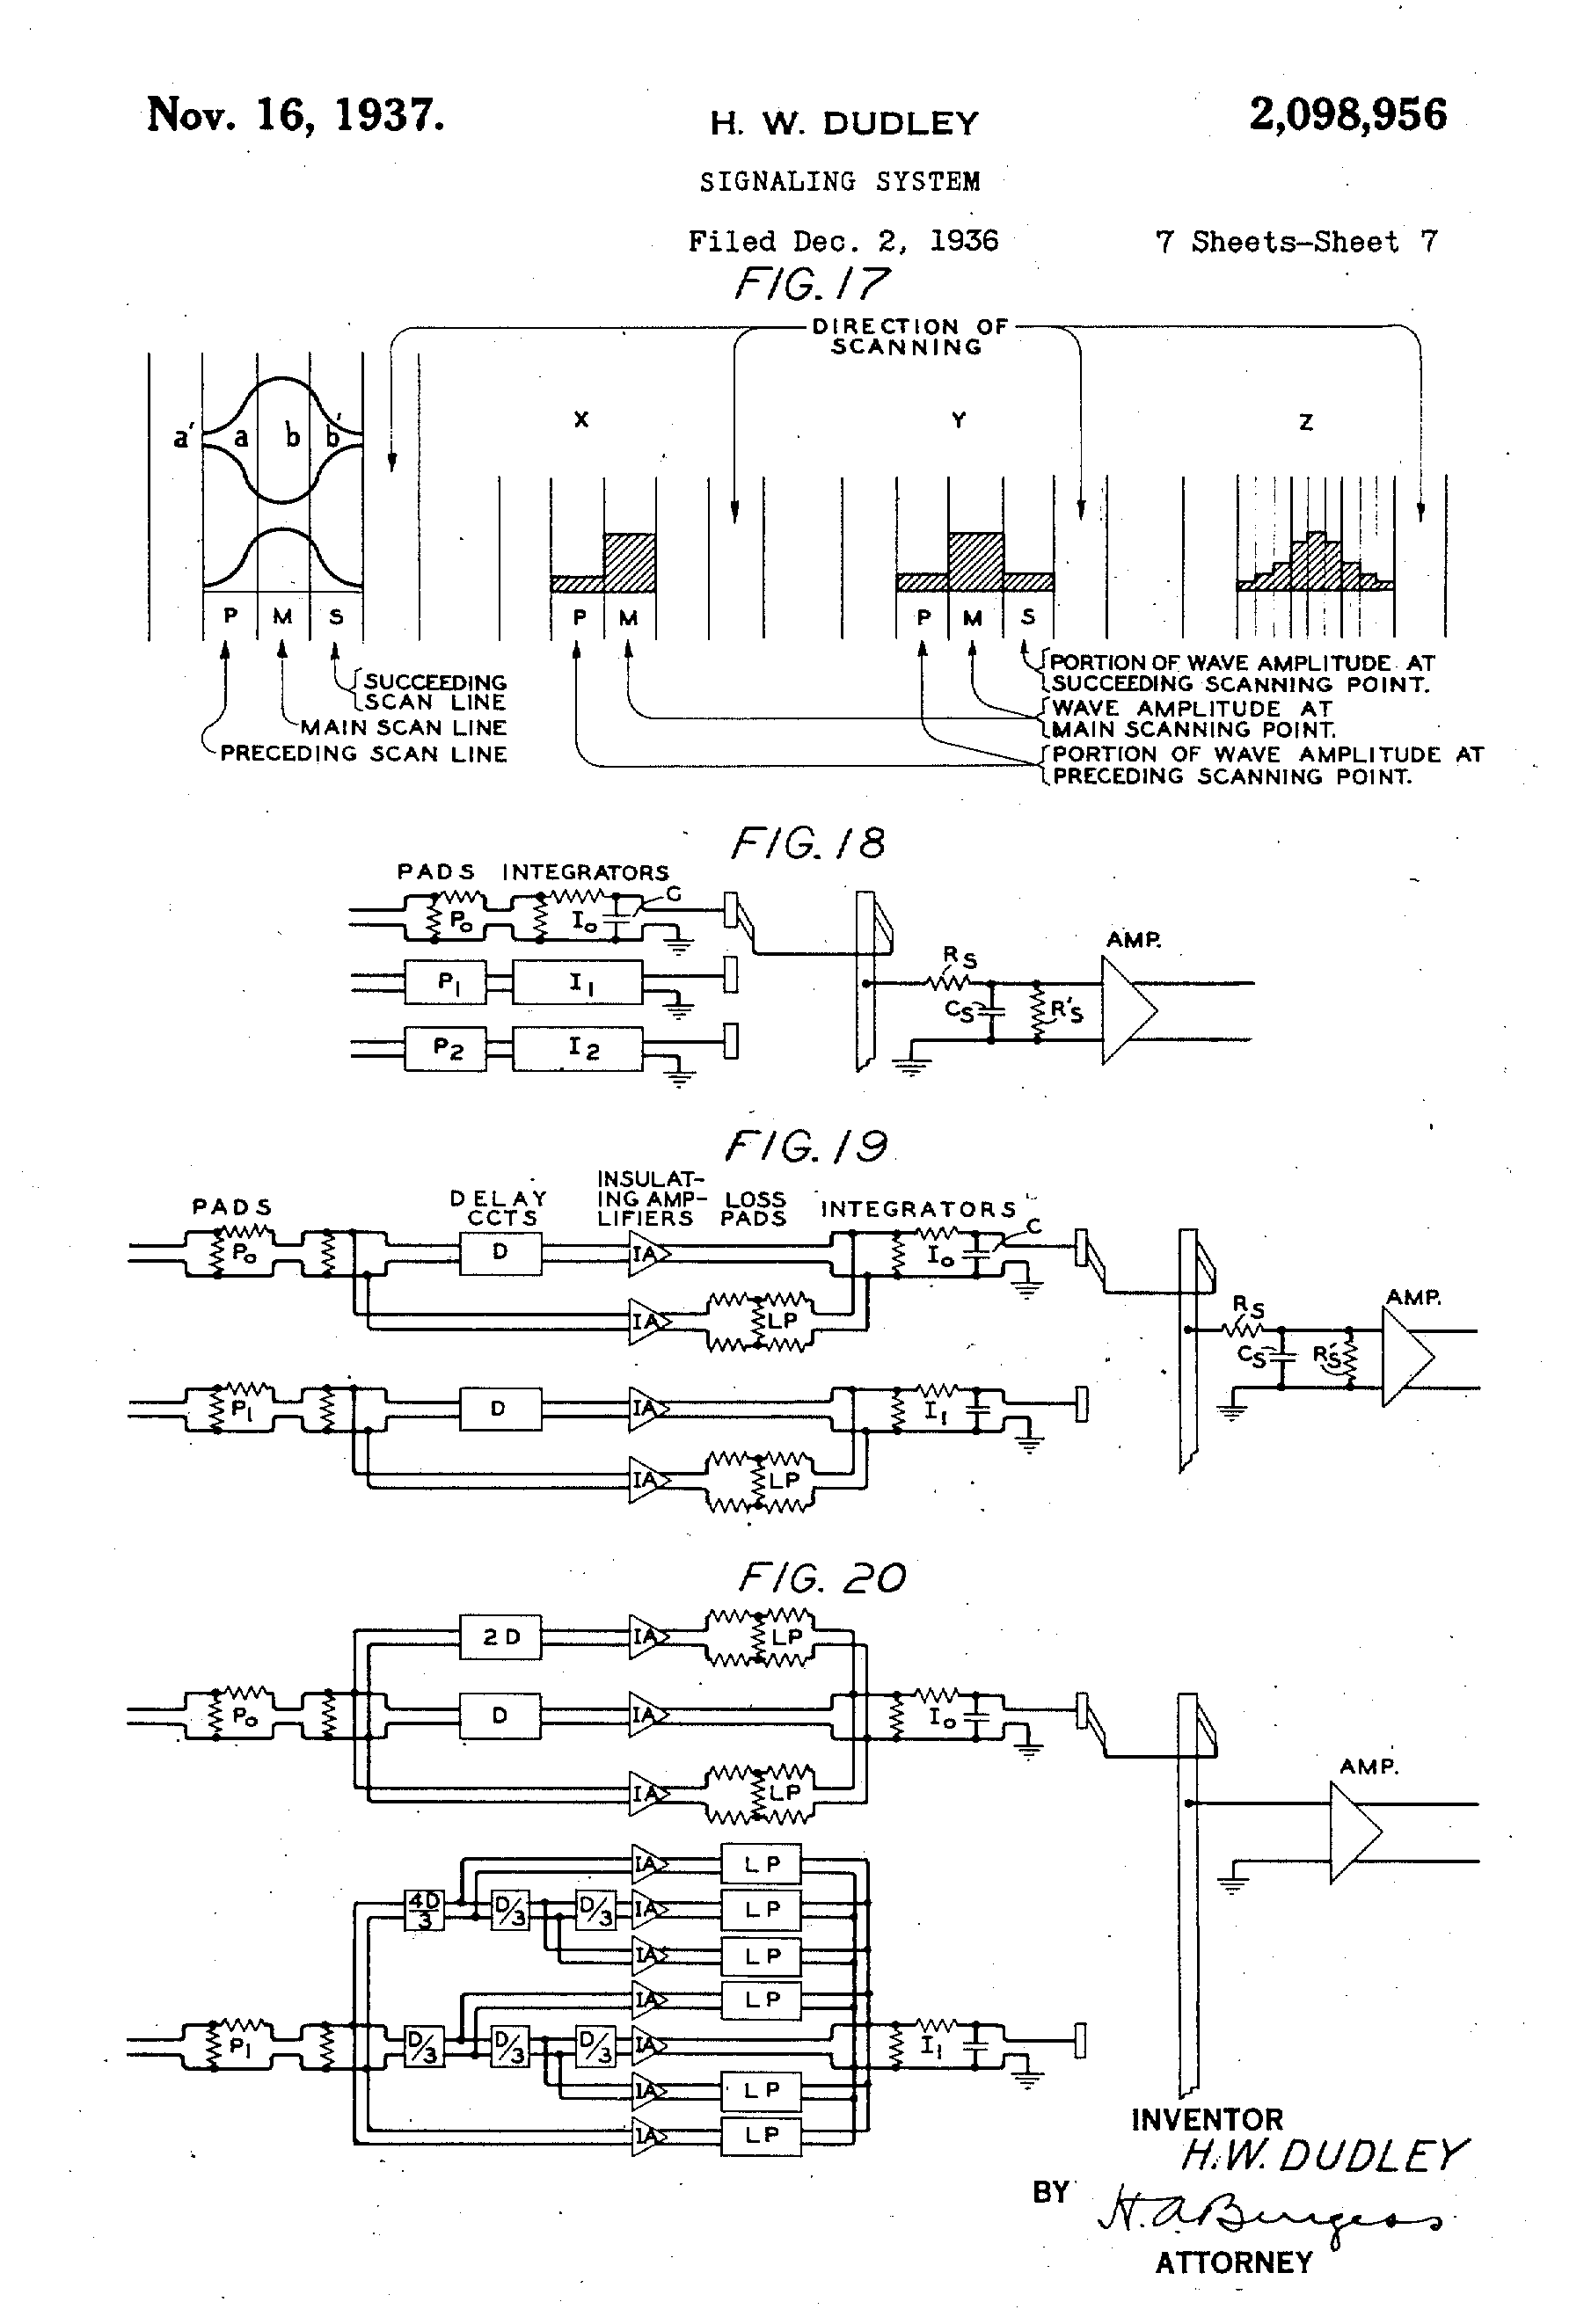
\includegraphics[height=0.8\textheight]{img/vocoder-patent.png}
    \caption{Bell Labs engineer Homer Dudley's 1937 patent (image: Google Patents)}
  \end{figure}
\end{frame}


\begin{frame}{Historical aside: Vocoders}
  \begin{figure}
    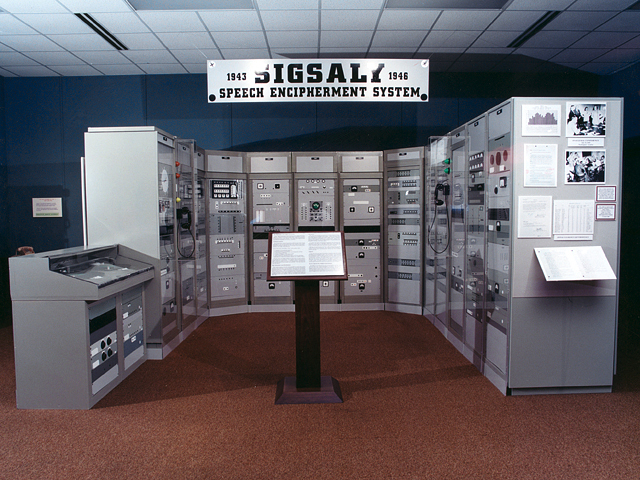
\includegraphics[width=0.8\textwidth]{img/sigsaly.jpg}
    \caption{SIGSALY - encrypted voice communications system used in WWII, built in 1943 by Bell Labs engineers (image: Wikipedia)}
  \end{figure}
\end{frame}

% Add animated gif of signal density using this technique:
% http://tex.stackexchange.com/questions/240243/getting-gif-and-or-moving-images-into-a-latex-presentation

    \begin{frame}{Temporal Resolution}
      \begin{figure}
      \animategraphics[loop,controls,width=\linewidth]{12}{img/audio_res/audio_res-}{0}{279}
      \caption{Using dialted convolutions, WaveNet is able to model raw waveforms at 16KHz (image: DeepMind)}
    \end{figure}
    \end{frame}

  \section{Architecture}
  \begin{frame}{Dilated convolutional layers}
    \begin{itemize}
      \item Causal, i.e. prediction $p(x_{t+1} | x_1, \dots, x_t)$ does not depend on future timesteps $x_{t+1}, \dots, x_T$.
      \item Filter is applied over an area larger than its length by skipping input values with a certain step
            \begin{itemize}
              \item Allows network to operate on a coarser scale than with a normal convolution, but more efficient
              \item A form of ``dimensionality reduction'' similar to pooling
            \end{itemize}
          \item Further reading 
            \begin{itemize}
            \item  Yu et al., ``Multi-Scale Context Aggregation by Dilated Convolutions'', ICLR 2016
            \item Chen et al., ``Semantic Image Segmentation with Deep Convolutional Nets and Fully Connected CRFs'', ICLR 2015
            \end{itemize}
    \end{itemize}
  \end{frame}

  \begin{frame}{Dilated convolutional layers}
    \begin{figure}
      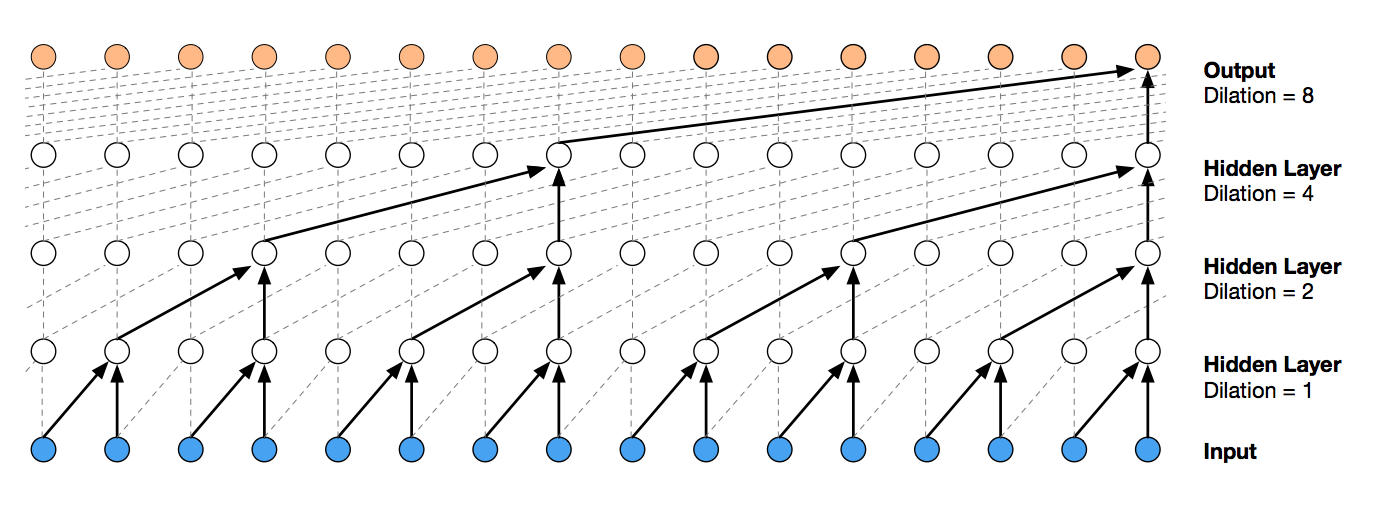
\includegraphics[width=\textwidth]{img/dilated_conv.png}
      \caption{Visualization of a stack of dilated convolutional layers}
    \end{figure}
    \begin{itemize}
    \item Stacked dilated convolutions enable very large receptive fields with few layers
    \end{itemize}
  \end{frame}

  \begin{frame}{Dilated convolutional layers}
    \begin{itemize}
      \item Let $F$ be a discrete function, and $k$ be a discrete filter of size $(2r+1)^2$.  The discrete convolution operator $*$ is defined as
        \[
          (F * k)(\mathbf{p}) = \sum_{\mathbf{s+t=p}} F(\mathbf{s}) k(\mathbf{t}).
        \]
        More generally, let $l$ be a dilation factor.  The $l$-dilated convolution can be defined as
        \[
          (F *_l k)(\mathbf{p}) = \sum_{\mathbf{s}+l\mathbf{t=p}} F(\mathbf{s}) k(\mathbf{t}).
        \]
      \item Implemented in TensorFlow as \texttt{tf.nn.atrous\_conv2d}
        \begin{itemize}
          \item Name comes from ``\`{a} trous'' in French, i.e. ``with holes''
        \end{itemize}
    \end{itemize}
  \end{frame}

  \begin{frame}{Dilated convolutional layers}
    \begin{itemize}
    \item Paper uses exponentially doubling dilations up to a limit, and then repeated:
      \[
        1,2,4,\dots,512,1,2,4,\dots,512,1,2,4,\dots,512.
      \]
     \item Each 1,2,4, \dots, 512 block has a receptive field of size 1024, a more efficient counterpart of $1 \times 1024$ convolution
      \item Stacking these units further increases model expressivity
    \end{itemize}
  \end{frame}

  \begin{frame}{Softmax distribution}
    \begin{itemize}
      \item Softmax empirically found to outperform mixture models (van den Oord et al. 2016) e.g. MCGSM\footnote{Theis et al., 2015} (even though audio waveforms are continuous)
      \item Raw audio typically stored as time series of 16-bit integer values (65,356 possibilities)
          \begin{itemize}
            \item Authors use a $\mu$-law companding transformation to quantize to 256 possible values
              \[
                f(x_t) = \sign(x_t) \frac{\ln(1 + \mu |x_t|)}{\ln (1 + \mu)},
              \]
              where $-1 < x_t < 1$ and $\mu = 255$.
            \item Well-known signal processing transform -- better reconstruction than linear quantization
          \end{itemize}
    \end{itemize}
  \end{frame}

  % Todo: try to add more motivation here
  \begin{frame}{Gated activation units}
    \begin{itemize}
      \item Gated activation units, same as used in gated PixelCNN (van den Oord et al., 2016)
        \[
          \mathbf{z} = \tanh(W_{f, k} * \mathbf{x}) \odot \sigma(W_{g, k} * \mathbf{x})
        \]
        \begin{itemize}
          \item $*$: convolution; $\odot$: elementwise multiplication
          \item $\sigma$: sigmoid function
          \item $k$: layer index; $f$: filter; $g$: gate
          \item $W$: learned convolution filter
        \end{itemize}
      \item Empirically found to outperform ReLUs
      \item Feedforward nets with gated units found beneficial in other works:
        \begin{itemize}
          \item Highway networks (Srivastava et al., NIPS 2015)
          \item Grid LSTM (Kalchbrenner et al. 2016, ICLR 2016)
          \item Neural GPUs (Kaiser et al. 2016, ICLR 2016)
        \end{itemize}
    \end{itemize}
  \end{frame}

  \begin{frame}{Residual / Skip Connections}
    \begin{figure}
      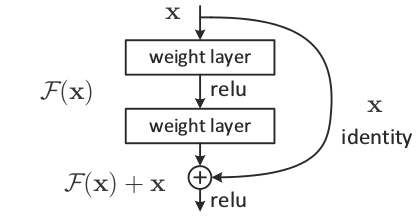
\includegraphics[width=0.6\textwidth]{img/residual_layer_he.png}
      \caption{Review: optimizing the residual $\mathcal{F}(\mathbf{x}) := \mathcal{H}(\mathbf{x}) - \mathbf{x}$ is more tractable for deeper networks (image: He et al. 2015)}
    \end{figure}
  \end{frame}

  \begin{frame}{Residual / Skip Connections}
    \begin{figure}
      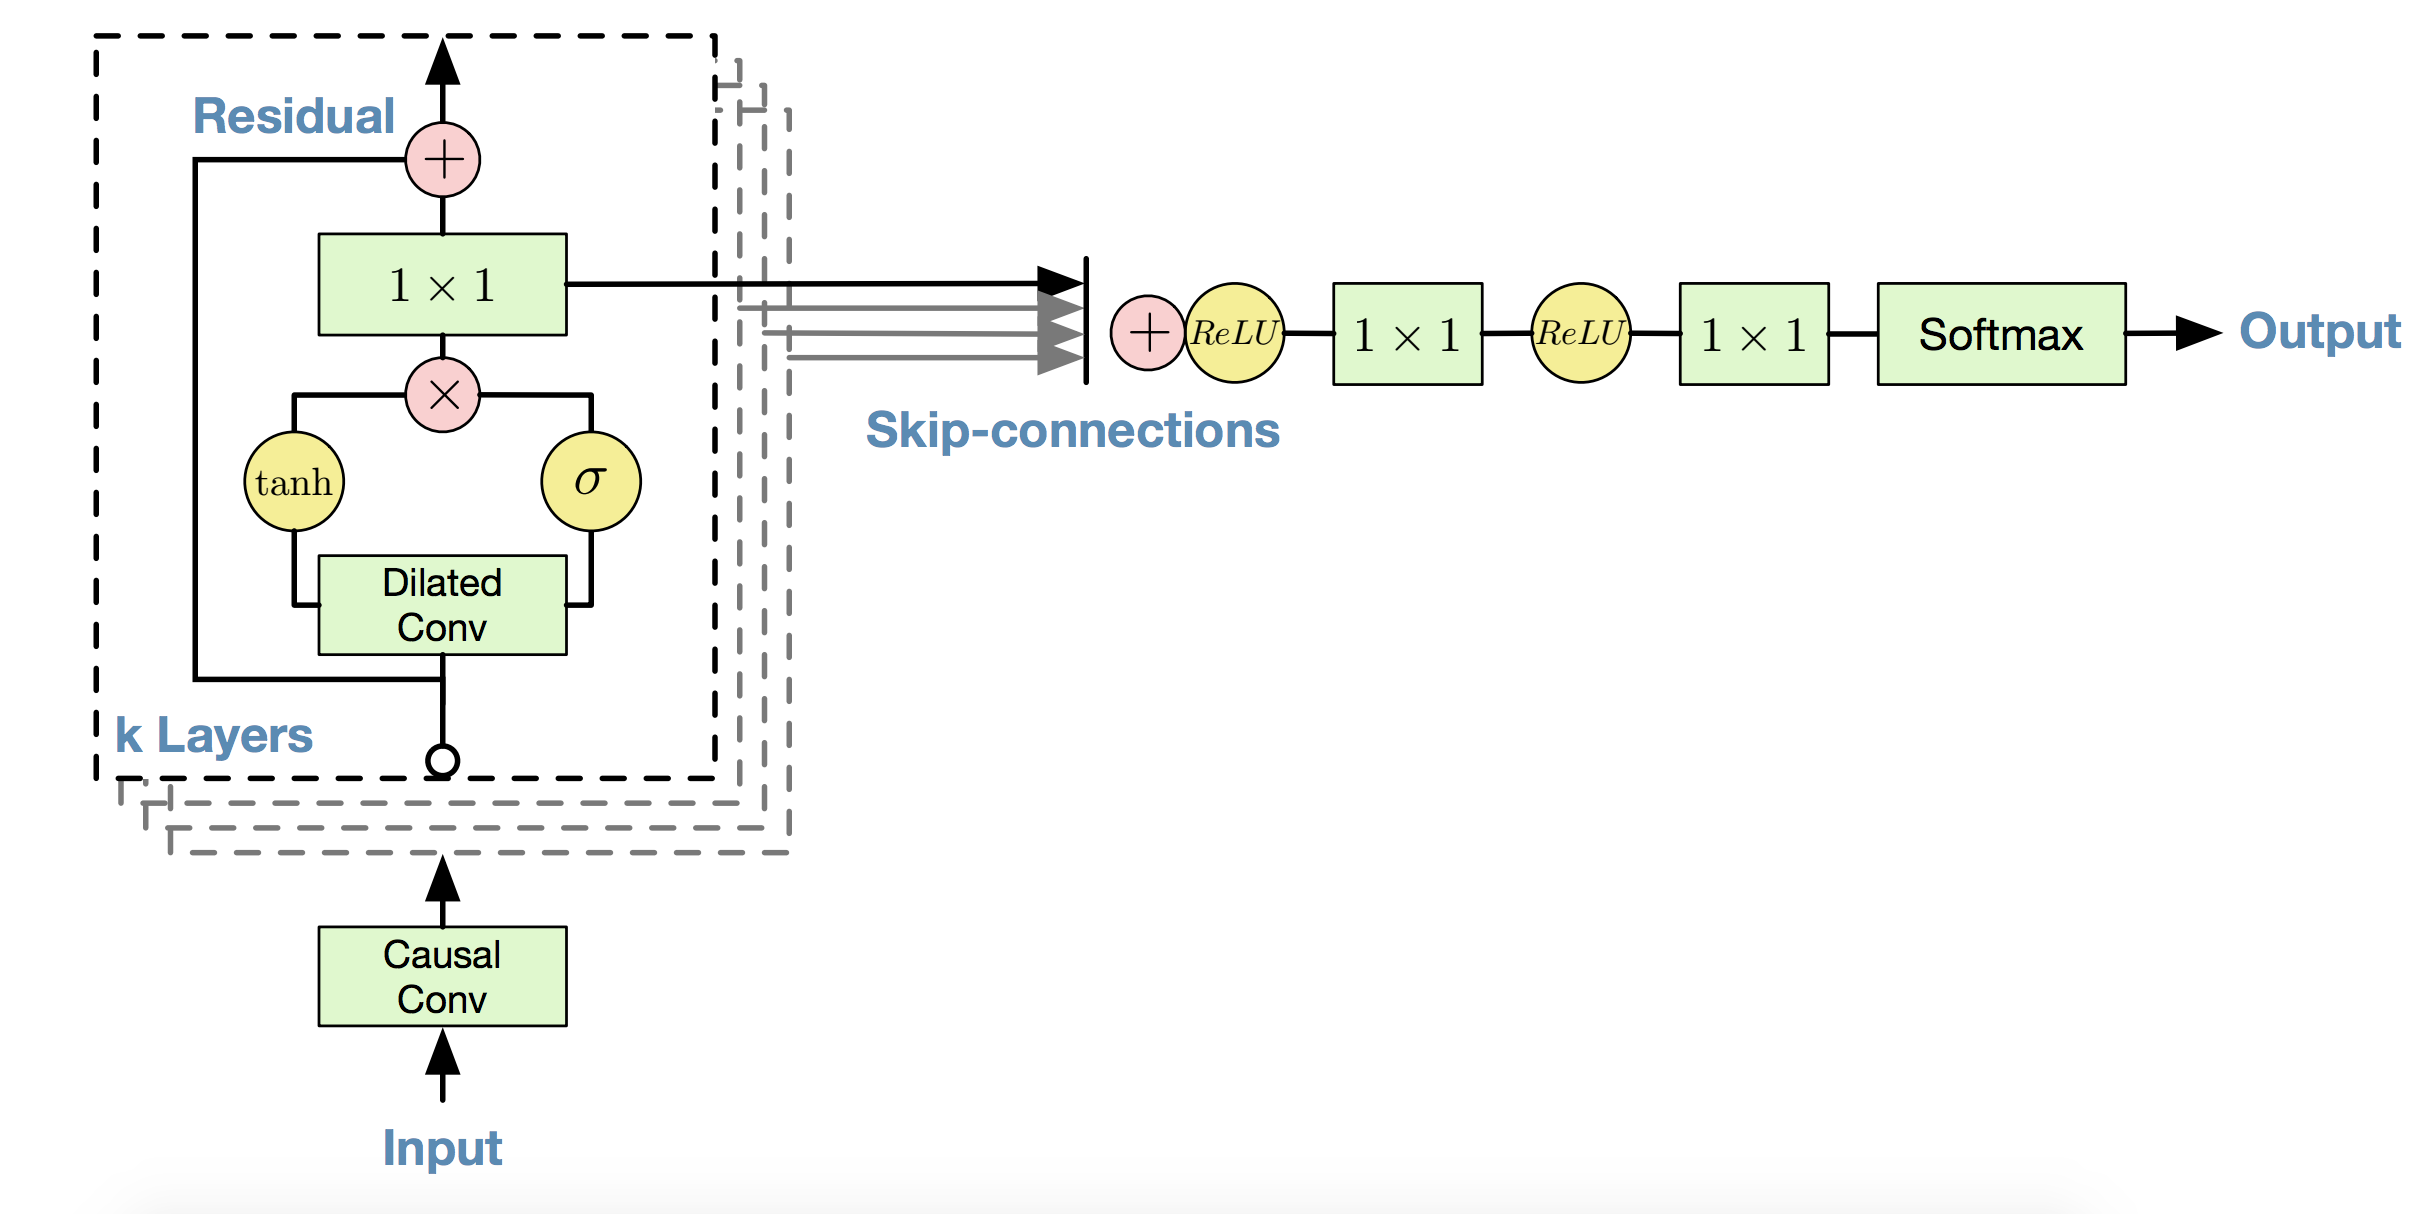
\includegraphics[width=1.0\textwidth]{img/residual_layer.png}
      \caption{summary of residual block and overall architecture}
    \end{figure}
  \end{frame}

  \begin{frame}{Conditional Wavenets}
    \begin{itemize}
      \item Given an aadditional $\mathbf{h}$, we model the conditional distribution $p(\mathbf{x} | \mathbf{h})$ of the waveform:
        \[
          p(\mathbf{x} | \mathbf{h}) = \prod_{t=1}^T p(x_t | x_1, \dots, x_{t-1}, \mathbf{h}).
        \]
     \item Conditioning on other variables enables audio generation with desired characteristics
     \item Examples: 
      \begin{itemize} 
       \item In multi-speaker setting, can pass in speaker identity
       \item For text-to-speech, can pass in information about text as extra input
      \end{itemize}
    \end{itemize}
  \end{frame}


  \begin{frame}{Global Conditioning}
    \begin{itemize}
      \item Can condition the model on other inputs in two different ways - global vs. local
      \item Global conditioning -- single latent variable $\mathbf{h}$ that influences output distribution across all timesteps (e.g. speaker embedding).    
      \item New activation function:
        \[
          \mathbf{z} = \tanh(W_{f, k} * \mathbf{x} + V_{f, k}^T \mathbf{h}) \odot (W_{g, k} * \mathbf{x} + V_{g, k}^T \mathbf{h}),
        \]
        where $V_{*, k}$ is a learned linear projection, and $V_{*, k}^T \mathbf{h}$ is broadcast over the time dimension.
    \end{itemize}
  \end{frame}

  \begin{frame}{Local Conditioning}
    \begin{itemize}
      \item Local conditioning - consider a second time series $h_t$, e.g. linguistic features in a TTS model

      \item First: upsample this time series using a transposed convolutional network.  Obtain new time series $\mathbf{y} = f(\mathbf{h})$, with same resolution as audio signal.

      \item New activation function:
        \[
          \mathbf{z} = \tanh(W_{f, k} * \mathbf{x} + V_{f, k} * \mathbf{y}) \odot \sigma(W_{g, k} * \mathbf{x} + V_{g, k} * \mathbf{y}),
        \]
        where $V_{f, k} * \mathbf{y}$ is now a $1 \times 1$ convolution.
    \end{itemize}
  \end{frame}

  \section{Experiments}
  \begin{frame}{Experiment A: Multi-speaker speech generation}

    \begin{itemize}
      \item Multi-speaker speech generation (free-form; not conditioned on text)
      \item Dataset: English multi-speaker corpus from CSTR voice cloning toolkit (VCTK)
        \begin{itemize}
          \item 44 hours of data from 109 different speakers
        \end{itemize}
     \item Conditioning on speaker with one-hot vector  
      \item Generated non-existent but human language-like words with realistic sounding intonations
        \begin{itemize}
          \item Analogous to ``realistic but unnatural'' generative models such as \url{http://karpathy.github.io/2015/05/21/rnn-effectiveness/}
        \end{itemize}
    \end{itemize}
  \end{frame}

  \begin{frame}{Experiment B: Text-to-speech}

    \begin{itemize}
      \item Dataset: Google's English (24.6 hours) / Mandain Chinese (34.8 hours) TTS corpus; professional female speakers
      \item Locally conditioned on linguistic features, derived from input texts
        \begin{itemize}
          \item Phone identities, syllable stress, number of syllables in a word, position of current syllable in phrase
          \item Computed every 5ms by phone-level alignment at train time
        \end{itemize}
      \item Also conditioned on logarithmic fundamental frequency $\log F_0$
      \item Receptive field size: 240 ms
    \end{itemize}
  \end{frame}

  \begin{frame}{Experiment B: Text-to-speech}
    \begin{figure}
      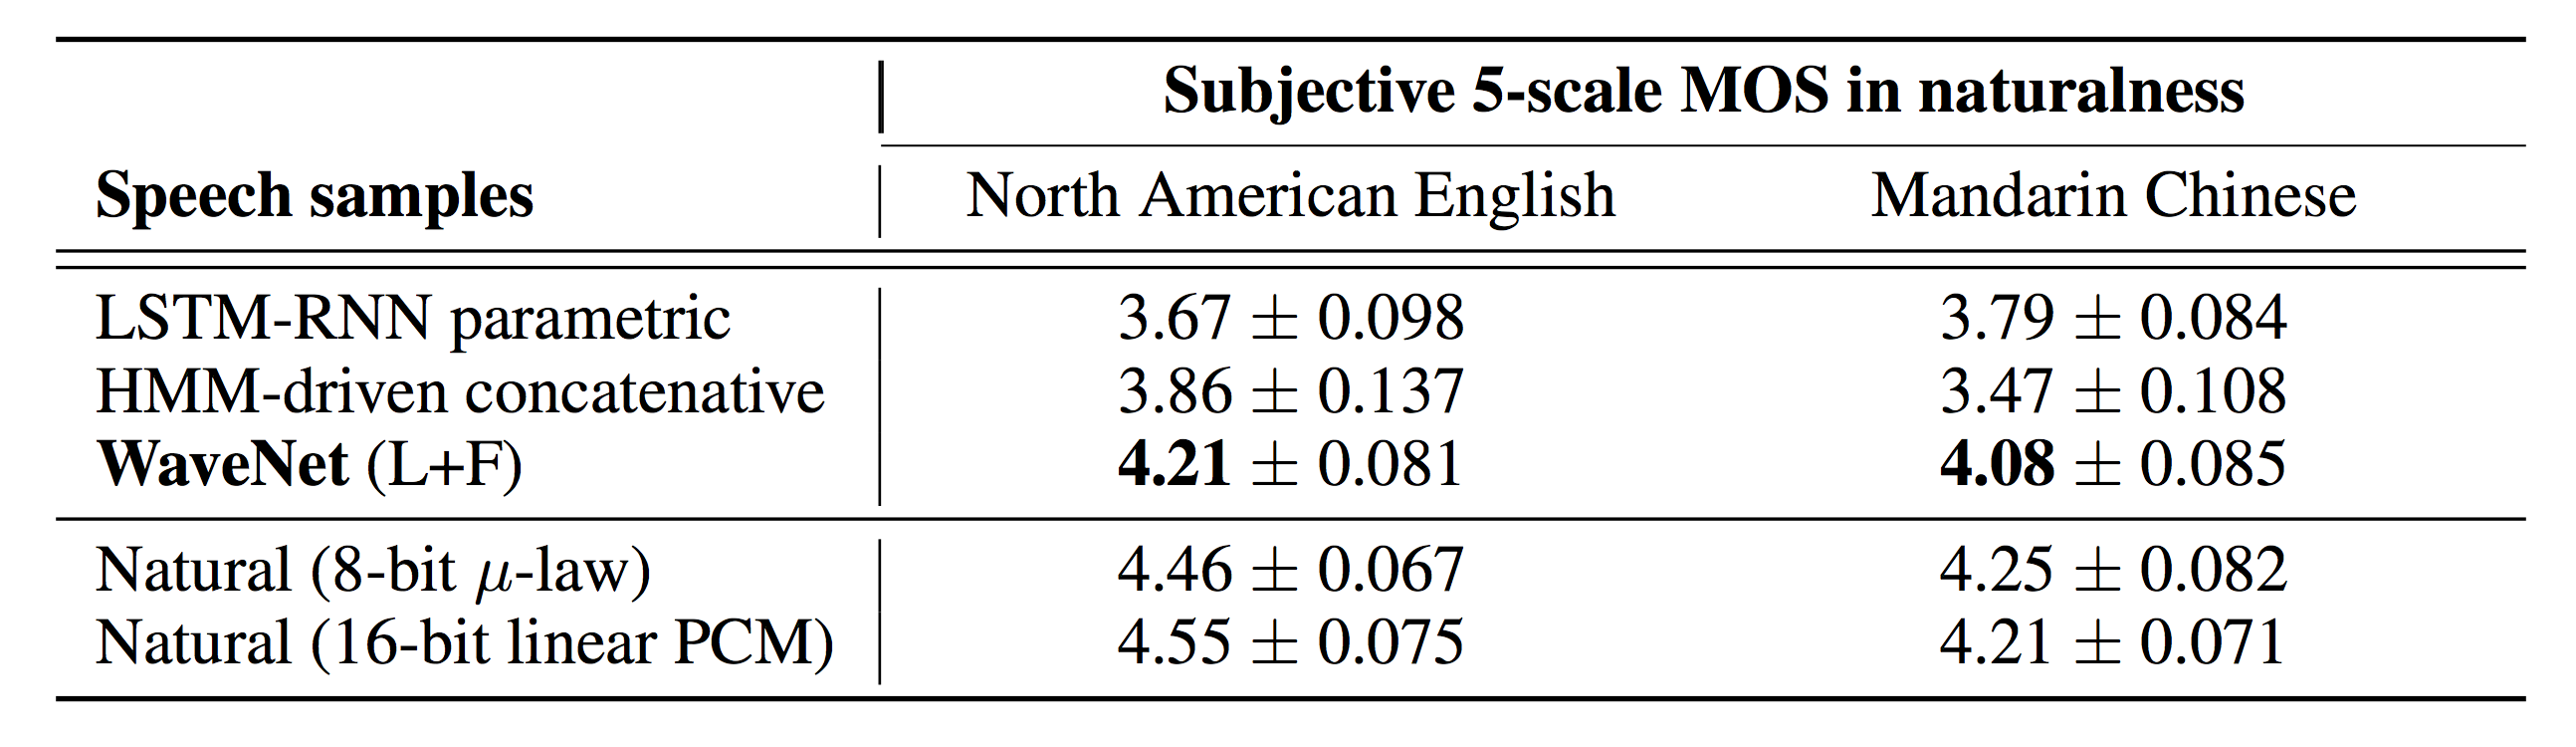
\includegraphics[width=1.0\textwidth]{img/exp_b.png}
      \caption{WaveNet outperforms mean opinion score in naturalness over LSTM / HMM models}
    \end{figure}
  \end{frame}

  \begin{frame}{Experiment C: Music generation}
    \begin{itemize}
        \item Datasets
          \begin{itemize}
            \item MagnaTagATune dataset (Law \& Von Ahn, 2009) --- 200 hours of audio, annotated with tags describing genre, instrumentation, tempo, volume, mood
            \item YouTube piano dataset --- 60 hours of solo piano music (easier to model, since constrained to a single instrument)
          \end{itemize}
        \item Key finding - enlarging receptive field was crucial to obtain samples that sound musical
        \item Authors conducted preliminary experiments conditioning on genre tags
    \end{itemize}
  \end{frame}

  \begin{frame}{Experiment D: Speech recognition}

  \begin{itemize}
    \item Speech recognition on the TIMIT dataset (Garafolo et al. 1993)
      \begin{itemize}
        \item 630 speakers
        \item Orthographic, phonetic, and word transcriptions
        \item 16-bit, 16kHz waveforms
      \end{itemize}
    \item Mean-pooling layer after dilated convolutions, activations over 10ms frames
    \item Loss consisted of two terms:
      \begin{itemize}
        \item Predicting the next sample
        \item Classify the frame
      \end{itemize}

    \item Achieved 18.8 PER on test set (state-of-the-art when trained on raw audio)

  \end{itemize}

  \end{frame}

  \begin{frame}{Further Reading} 
    \begin{itemize}
      \item Oord, Aaron van den, et al. "Conditional Image Generation with PixelCNN Decoders." arXiv preprint arXiv:1606.05328 (2016).
      \item  Oord, Aaron van den, Nal Kalchbrenner, and Koray Kavukcuoglu. "Pixel recurrent neural networks." arXiv preprint arXiv:1601.06759 (2016).
        
      \item Salimans, Tim, et al. "PixelCNN++: Improving the PixelCNN with Discretized Logistic Mixture Likelihood and Other Modifications." arXiv preprint arXiv:1701.05517 (2017).
      \item Gulrajani, Ishaan, et al. "PixelVAE: A Latent Variable Model for Natural Images." arXiv preprint arXiv:1611.05013 (2016).
      \item Mehri, Soroush, et al. "SampleRNN: An Unconditional End-to-End Neural Audio Generation Model." arXiv preprint arXiv:1612.07837 (2016).
        
    \end{itemize}
  \end{frame}

\end{document}
